\section{a) False position method}

\subsection{Problem}

We have to find zeros of the function
\[ f(x) = -2.1 + 0.3x - xe^{-x} \]
In the interval $[-5; 10]$ using false position method.

\subsection{Theoretical Introduction}
\emph{False position} method also called \emph{regula falsi} in fancier circles is similar to the bisection method, the difference is that the interval we use $[a_n, b_n]$ is divided into two subintervals. We have:
\begin{itemize}
\item $\alpha$ - The root
\item $a_n$ - 'left' interval
\item $b_n$ - 'right' interval
\item $f(a_n)$ - Value at left interval
\item $f(b_n)$ - Value at right interval
\end{itemize}

We get:
\[ \frac{f(b_n) - f(a_n)}{b_n - a_n} = \frac{f(b_n) - 0}{b_n - c_n} \]
From which we get:
\[ c_n = b_n - \frac{f(b_n)(b_n - a_n)}{f(b_n) - f(a_n)} = \frac{a_nf(b_n) - b_n f(a_n)}{f(b_n)-f(a_n)} \]

Then we choose next interval as in the bisection method so: we calculate products of function values at $a_n$ and $b_n$ and that subinterval is selected for the next iteration of \emph{false position} method. This subinterval corresponds to the negative product value.

\subsubsection{Properties of \emph{false position method}}
This method is always convergent, simillary to bisection method, since it will always choose and shorten the interval which contains the root. If the function is continous and differentiable the method is linearly convergent. That being said the convergence may become sluggish. It can happen if for example one of the endpoints of the intervals will remain the same and the iterating will not shorten the interval to 0. One of the examples of functions that lead to that are barrier functions used in constrained optimization methods.

\paragraph{Improvement to the method}
In order to improve the formula and avoid aforementioned situation we can take smaller value of the function for the value that does not change.
For right end:
\[ c_n = \frac{a_n\frac{f(b_n)}{2} - b_nf(a_n)}{\frac{f(b_n)}{2} - f(a_n)} \]
And for left end:
\[ c_n = \frac{a_nf(b_n) - b_n\frac{f(a_n)}{2}}{f(b_n)- \frac{f(a_n)}{2}} \]

This is called \emph{modified regula falsi} or \emph{Illinois algorithm}.
It is superlinearly convergent, globally convergent and length of intervals we get in each iterations converges to zero.
\subsection{Results}

\begin{center}
   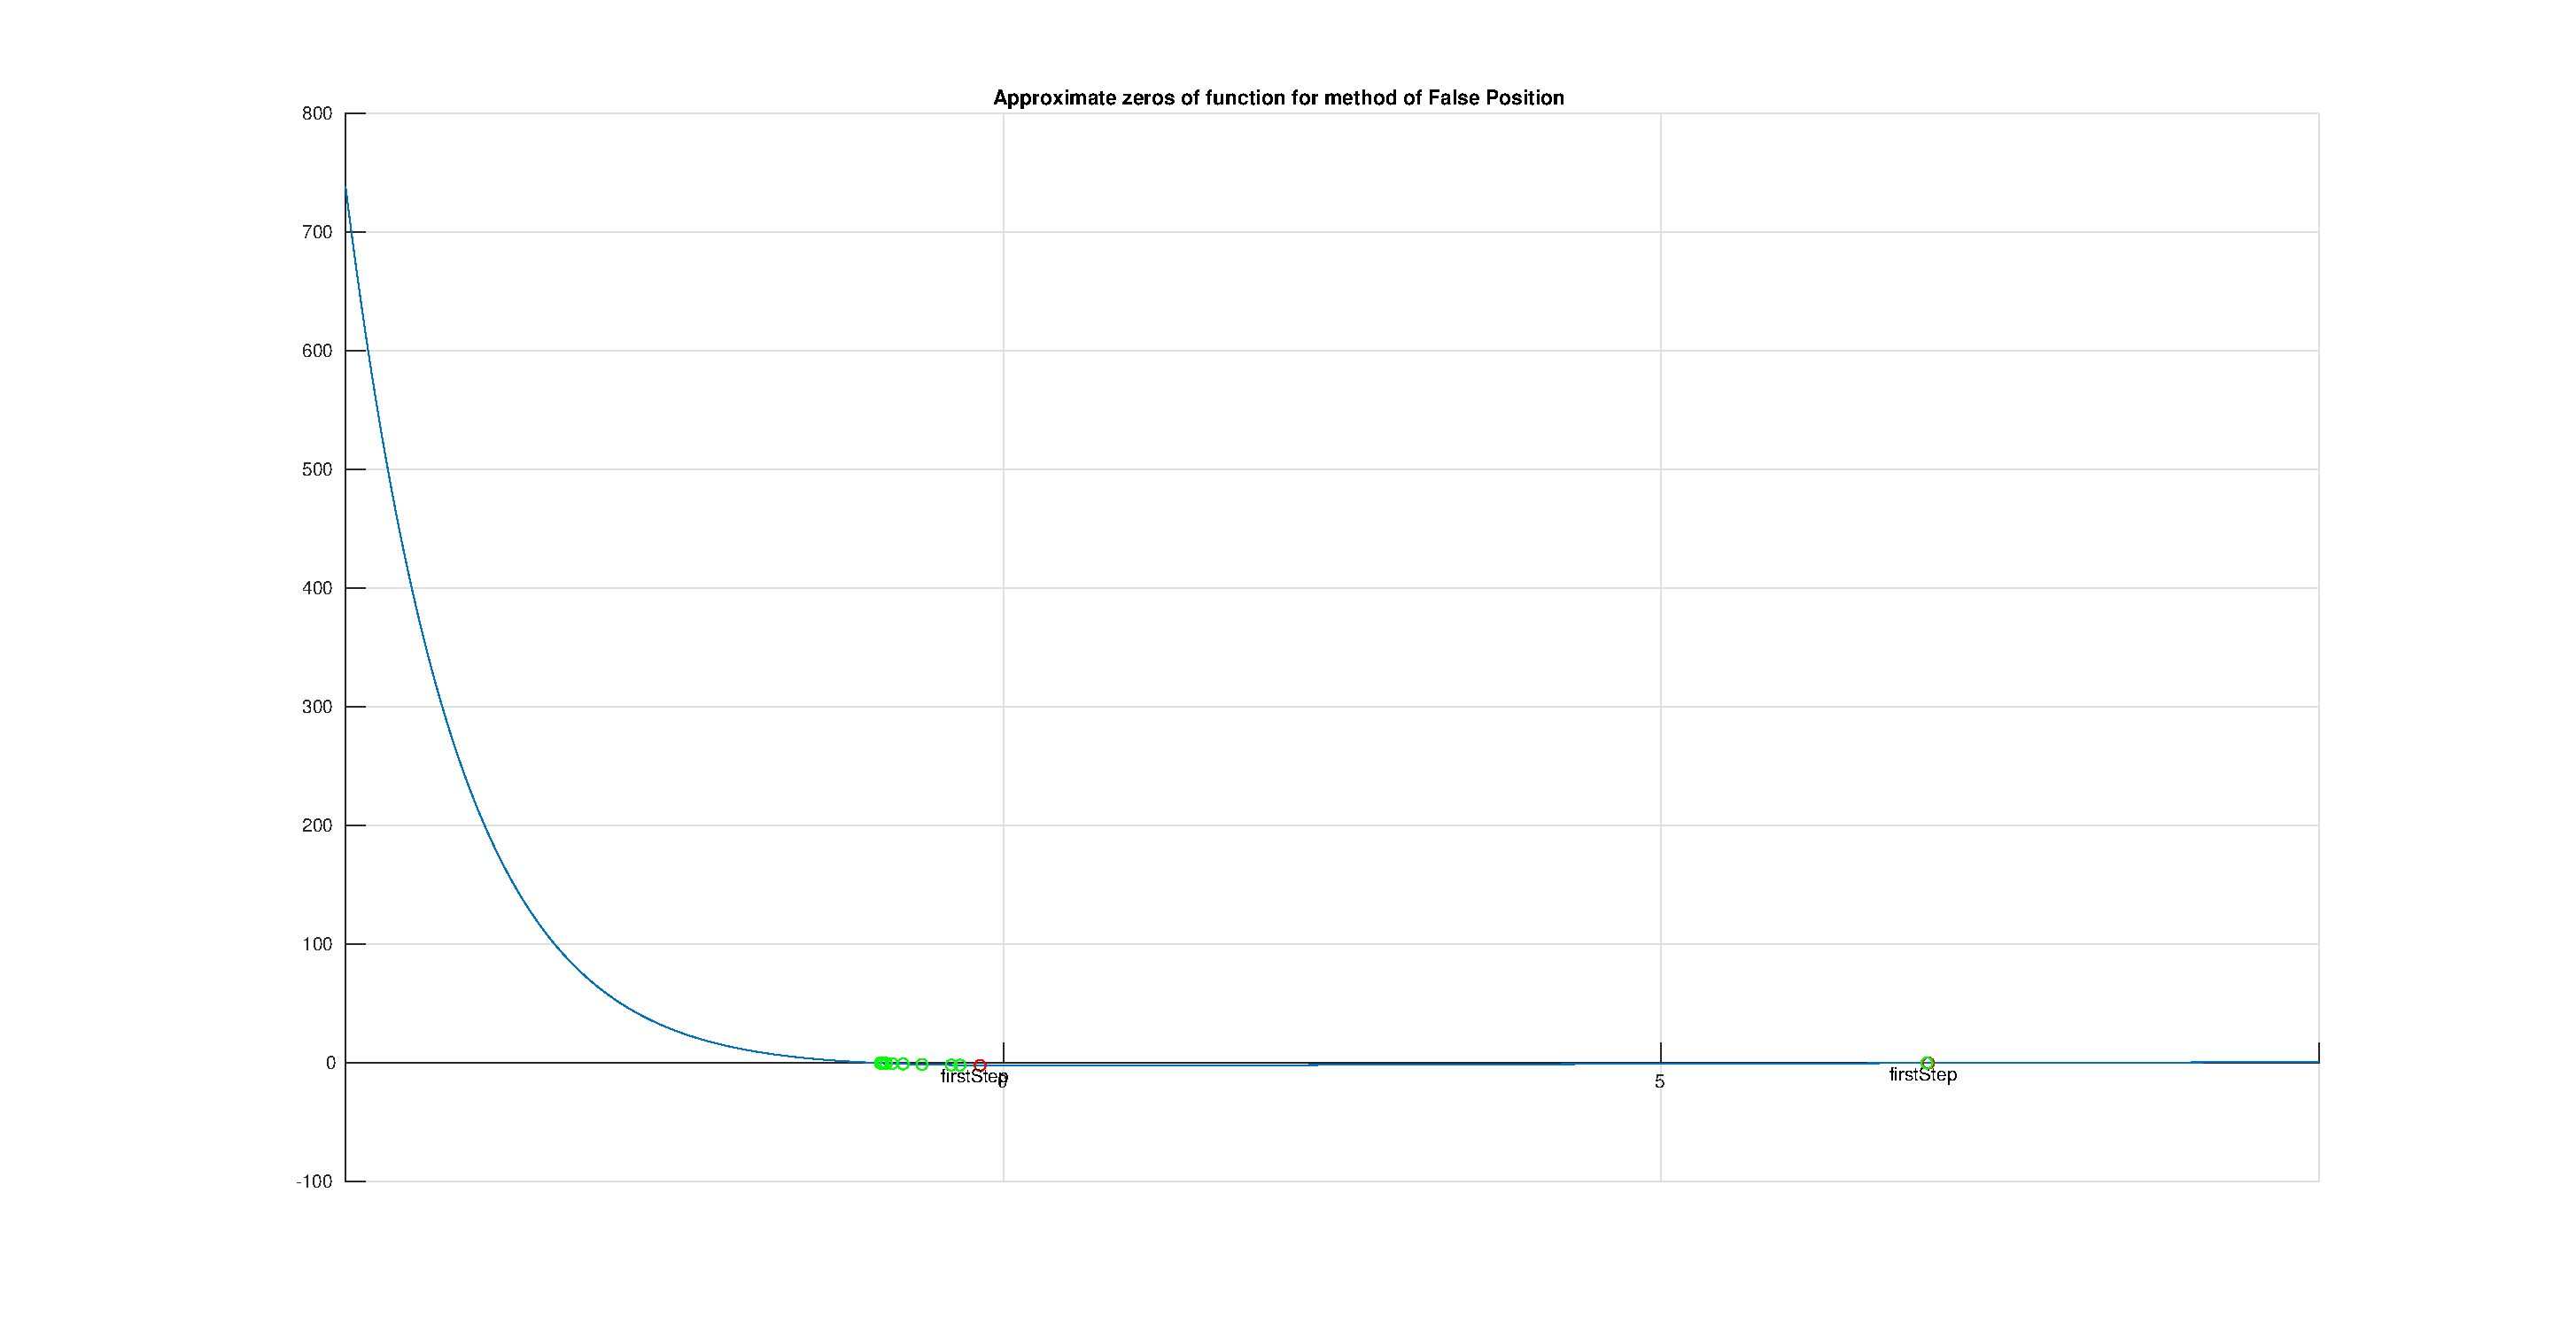
\includegraphics[scale=0.25]{task1falsepositionoverall.eps}
\end{center}

\begin{center}
   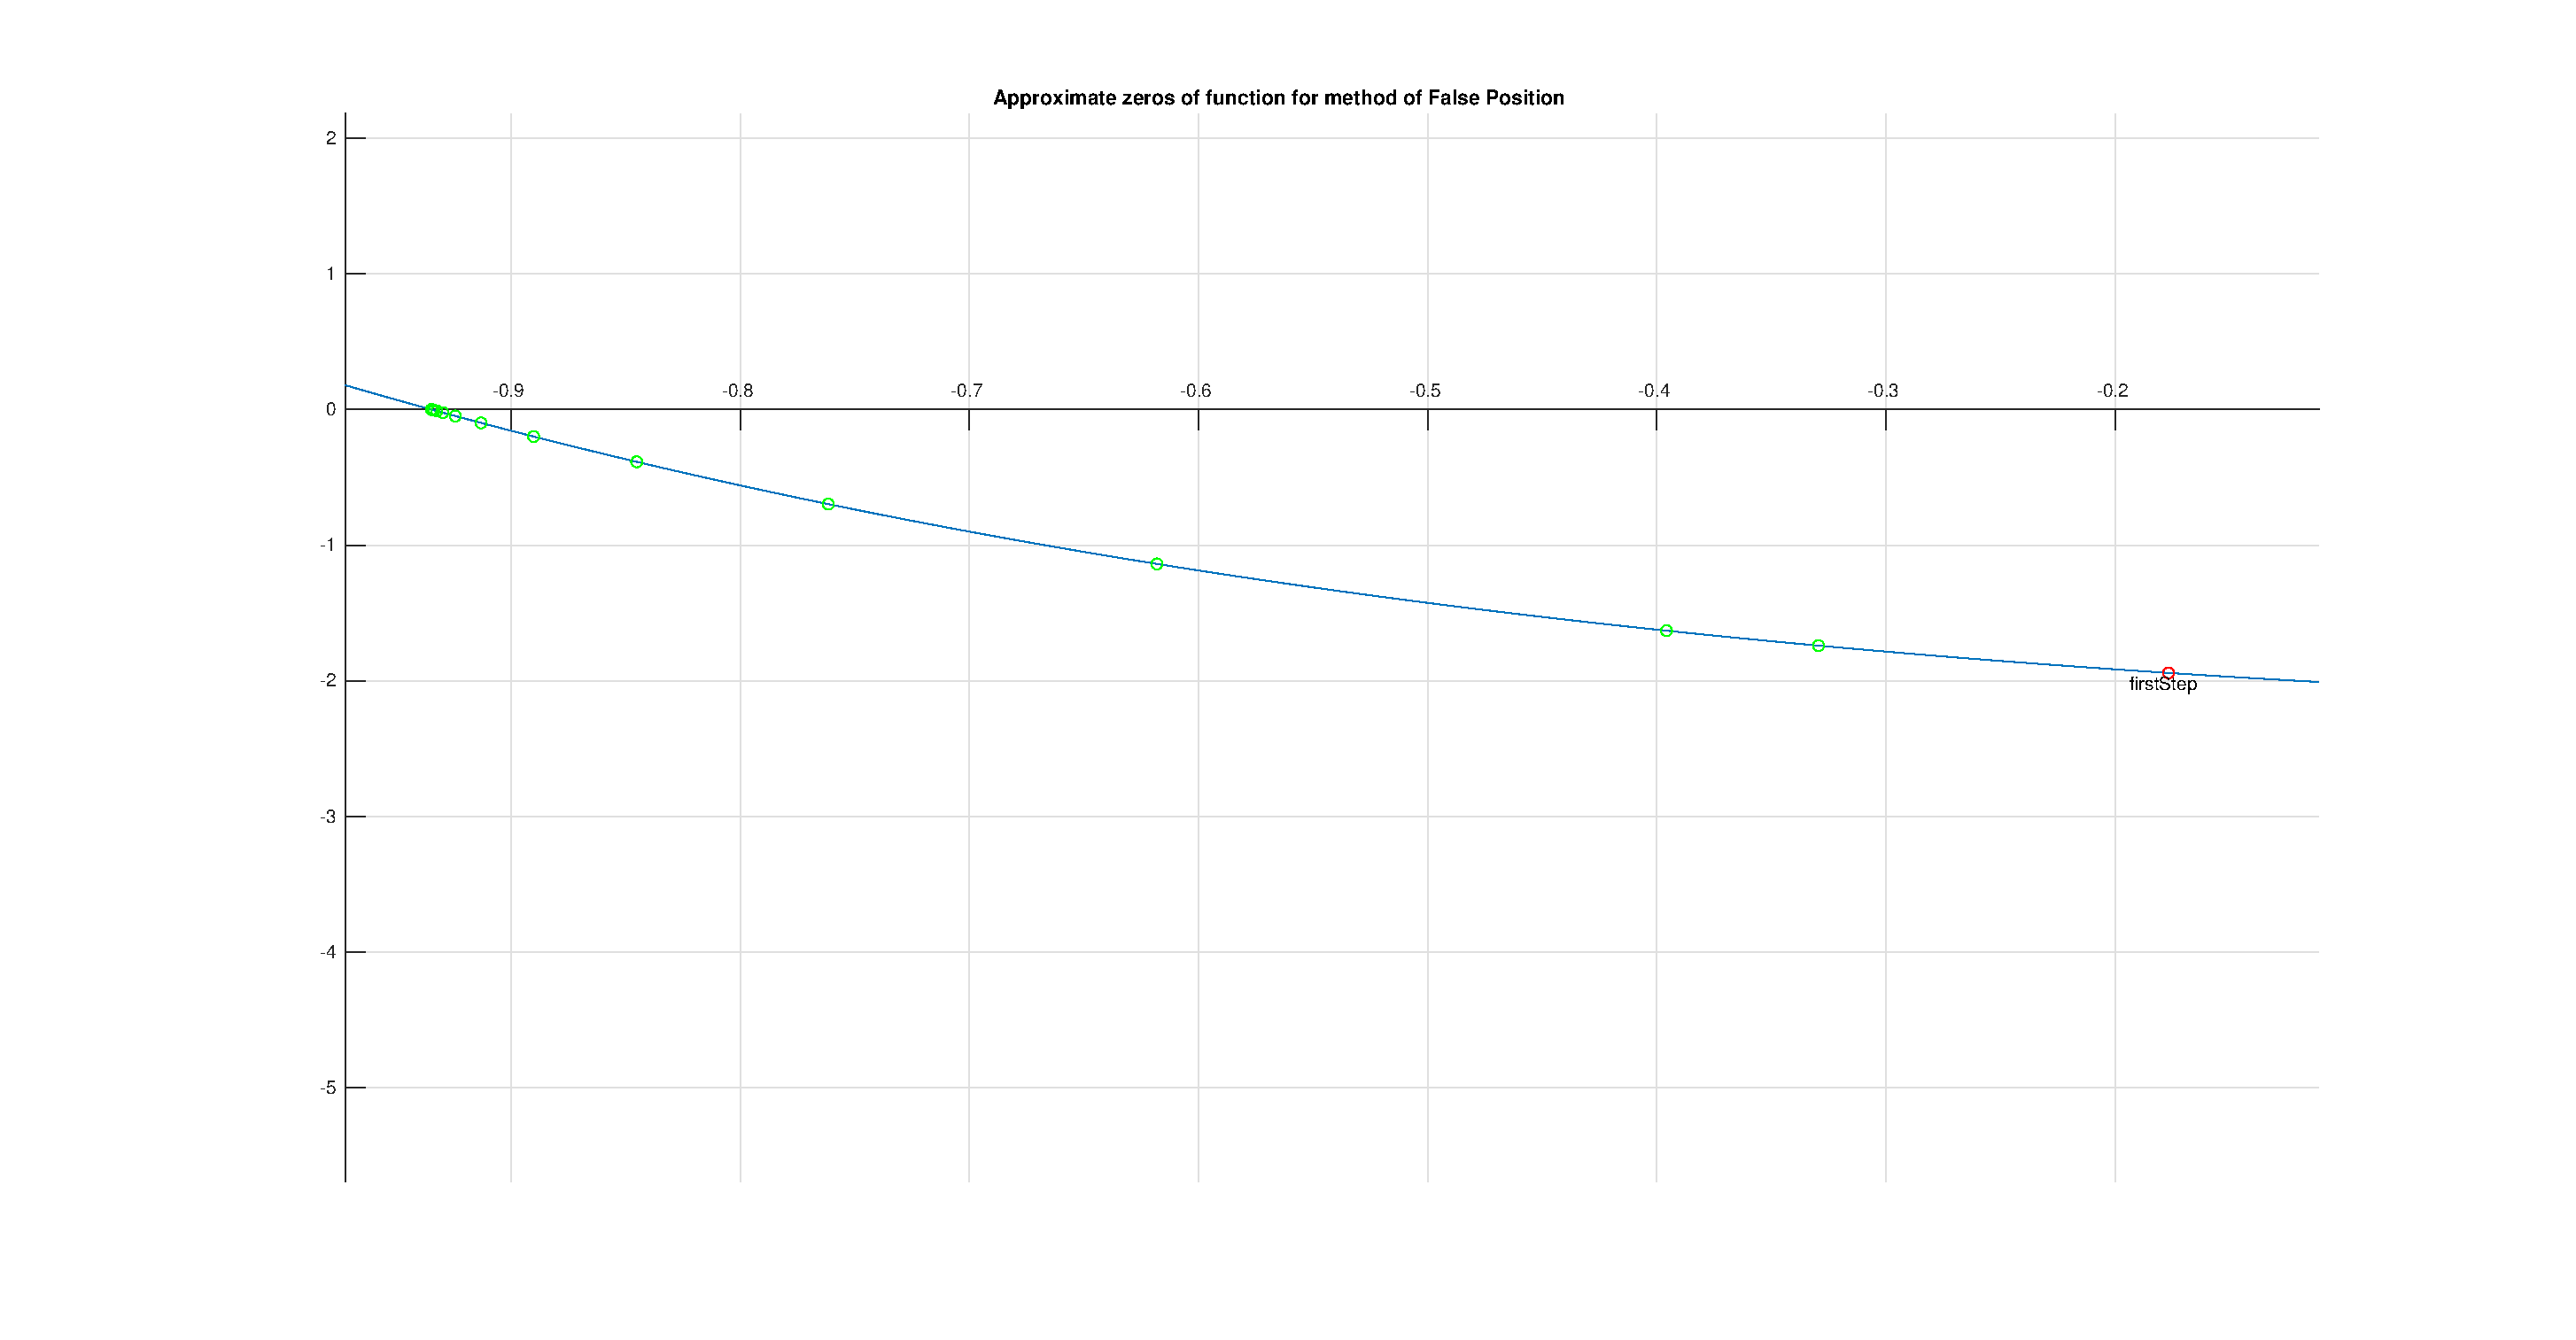
\includegraphics[scale=0.25]{task1falsepositionzommedleft.eps}
\end{center}

\begin{center}
   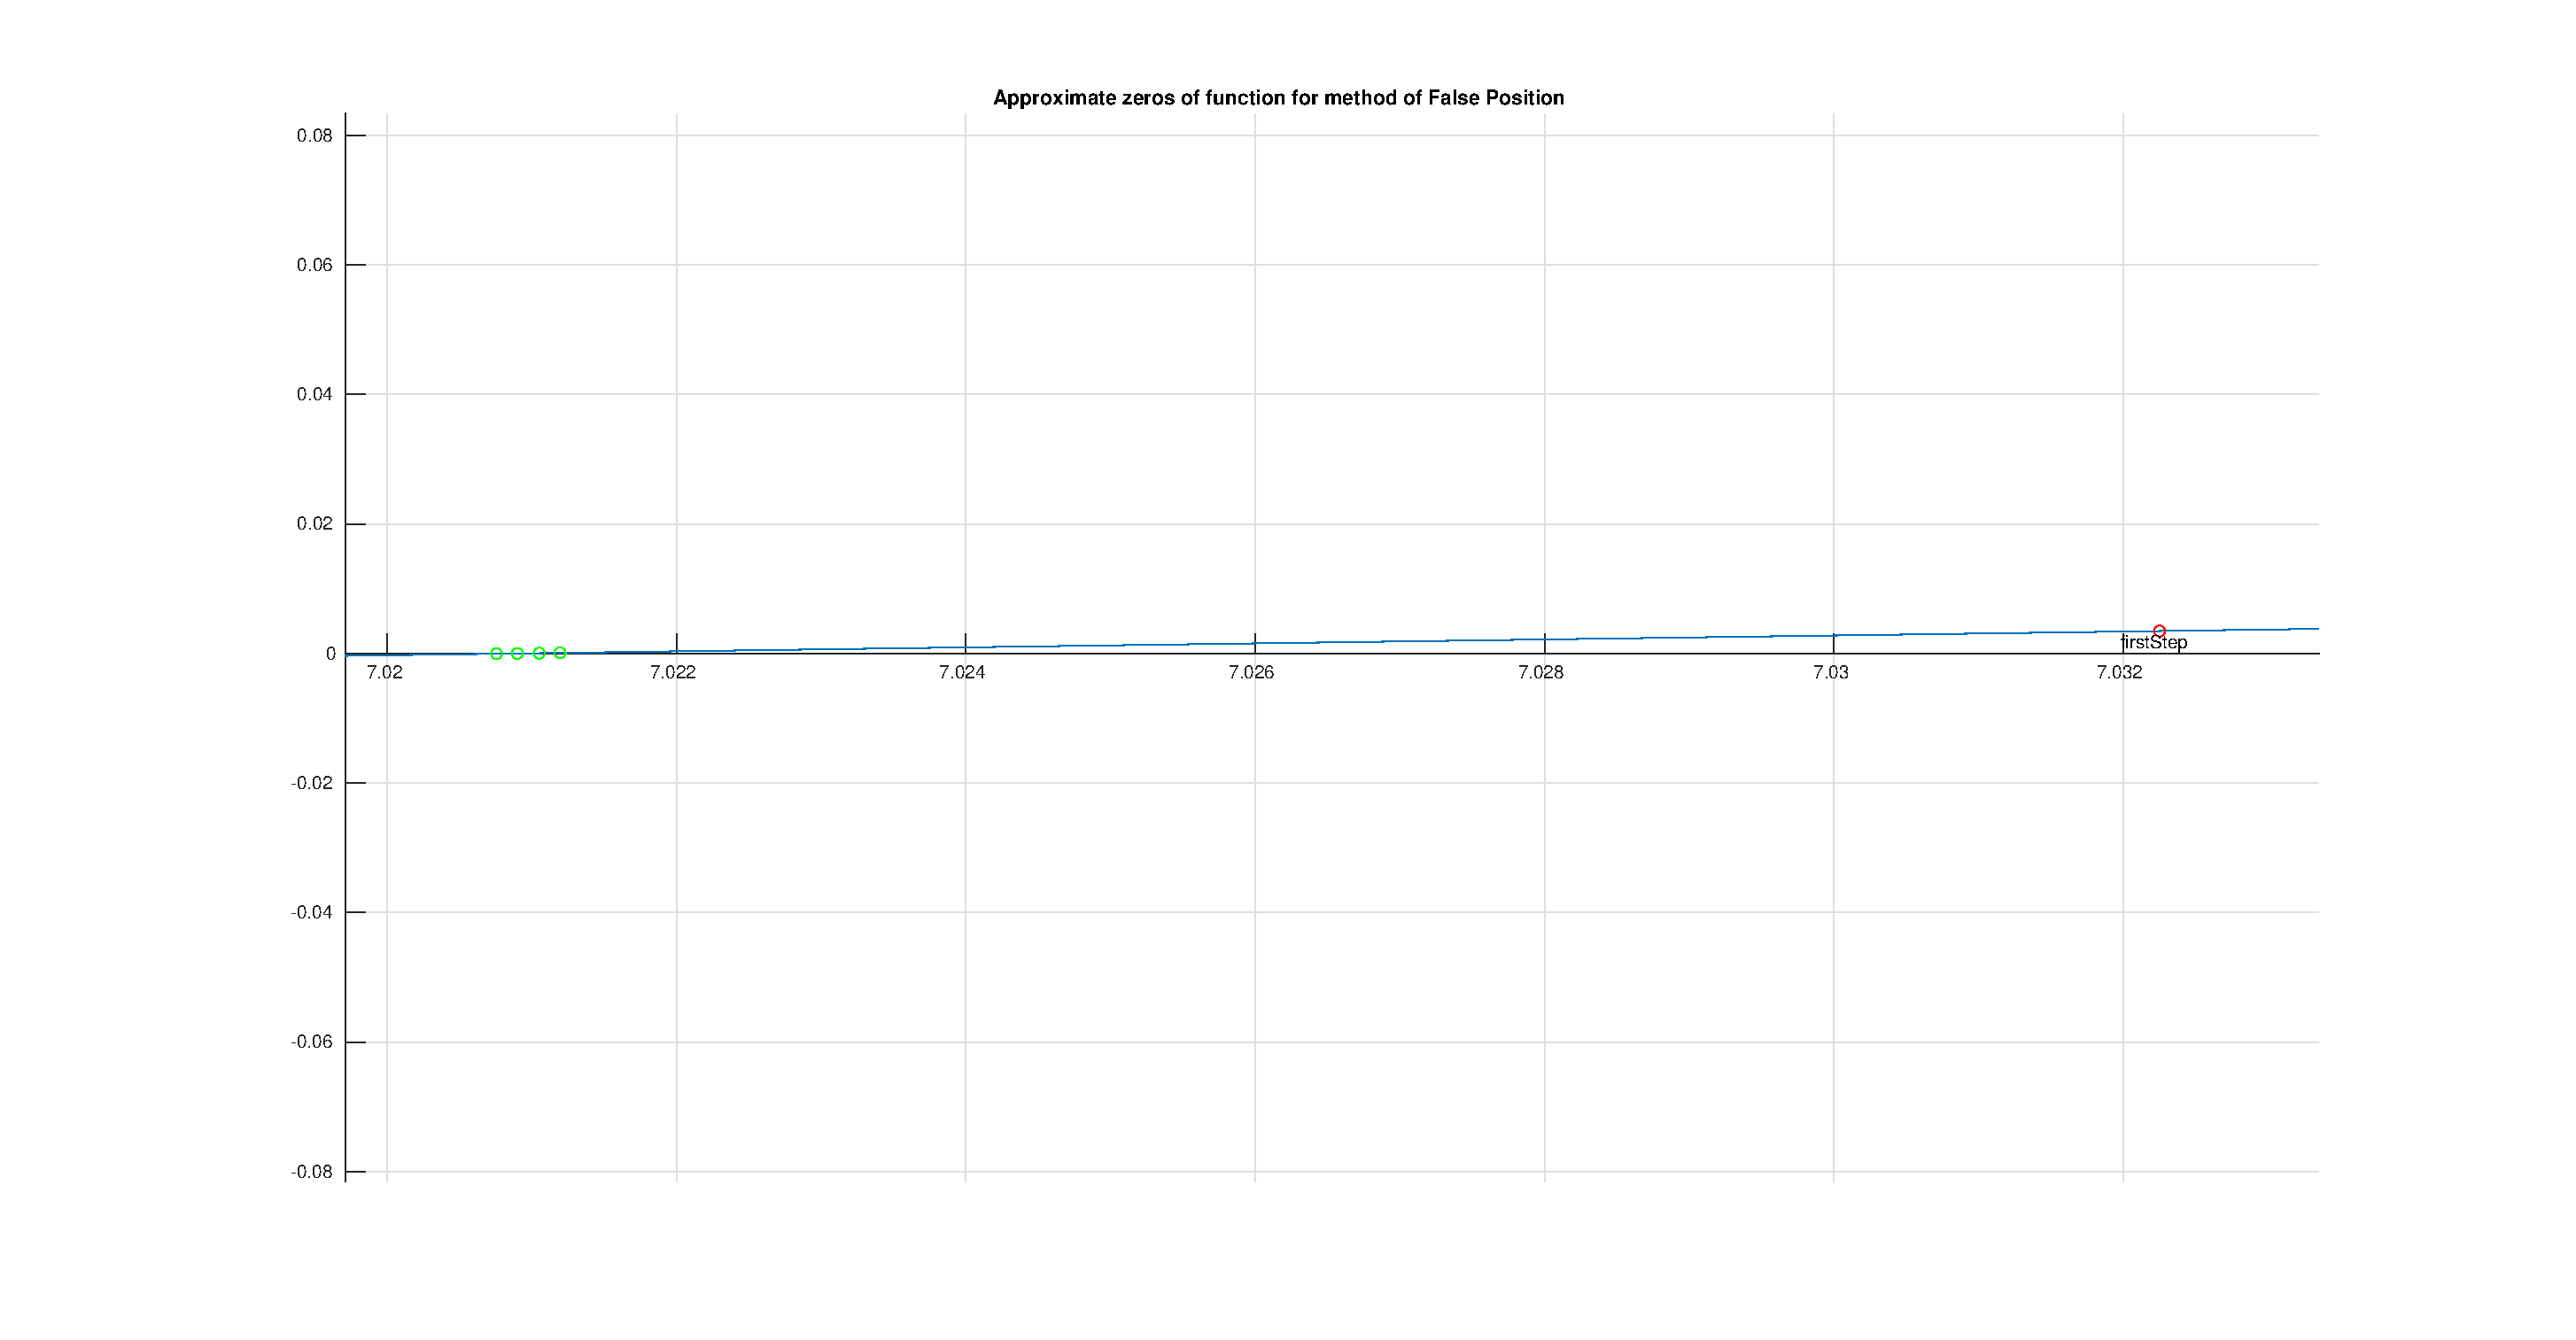
\includegraphics[scale=0.25]{task1falsepositionzommedright.eps}
\end{center}

\begin{center}
  \begin{tabular}{| c  c c |}
\hline
Iteration & root         & f(root) \\
\hline
1   &  -0.17673         &-1.9421 \\
\hline
2   &  -0.32943         &-1.7409 \\
\hline
3    & -0.39578         &-1.6308 \\
\hline
4     &-0.61812         &-1.1386 \\
\hline
5     &-0.76152        &-0.69765 \\
\hline
6     &-0.84516        &-0.38573 \\
\hline
7     &-0.89015        &-0.19911 \\
\hline
8     &-0.91304       &-0.098733 \\
\hline
9    & -0.92431       &-0.047922 \\
\hline
10    & -0.92976       & -0.02301 \\
\hline
11     &-0.93237       & -0.01099 \\
\hline
12     &-0.93362       &-0.005236 \\
\hline
13     &-0.93421      &-0.0024915 \\
\hline
14      &-0.9345      &-0.0011848 \\
\hline
15     &-0.93463      &-0.0005633 \\
\hline
16     &-0.93469     &-0.00026777 \\
\hline
17     &-0.93473     &-0.00012728 \\
\hline
18     &-0.93474     &-6.0499e-05 \\
\hline
19     &-0.93475     &-2.8756e-05 \\
\hline
20     &-0.93475    & -1.3668e-05 \\
\hline
21     &-0.93475    & -6.4964e-06 \\
\hline
22     &-0.93475    & -3.0878e-06 \\
\hline
23     &-0.93475    & -1.4676e-06 \\
\hline
24     &-0.93475    & -6.9758e-07 \\
\hline
25     &-0.93475    & -3.3157e-07 \\
\hline
26     &-0.93475    & -1.5759e-07 \\
\hline
27     &-0.93475    & -7.4906e-08 \\
\hline
28     &-0.93475    & -3.5603e-08 \\
\hline
29     &-0.93475    & -1.6922e-08 \\
\hline
30     &-0.93475    & -8.0433e-09 \\
\hline
31     &-0.93475    &  -3.823e-09 \\
\hline
32     &-0.93475    & -1.8171e-09 \\
\hline
33     &-0.93475    & -8.6368e-10 \\
\hline
34     &-0.93475    & -4.1051e-10 \\
\hline
35     &-0.93475    & -1.9512e-10 \\
\hline
36     &-0.93475    & -9.2741e-11 \\
\hline
\end{tabular}
\end{center}

\begin{center}
  \begin{tabular}{| c  c c |}
\hline
Iteration & root         & f(root) \\
\hline
1   &  7.0323         & 0.0034663 \\
\hline
2   &  7.0212          & 9.0344e-05 \\
\hline
3    & 7.0211         & 4.6349e-05 \\
\hline
4     & 7.0208        & -4.3921e-05  \\
\hline
5     & 7.0209        & 4.8939e-11  \\
\hline

\hline
\end{tabular}
\end{center}

